\documentclass{protokol}
\leftheader{Lom světla, disperze}
\centerheader{Praktikum III}
\rightheader{Tomáš Derner}

\begin{document}

  \section*{Úkol}

    \begin{enumerate}
      \item Změřte index lomu a střední disperzi přiložené kapaliny v závislosti na koncentraci (stačí 5 různých koncentrací).
      \item Změřte indexy lomu tří optických skel.
      \item Změřte index lomu řádného paprsku a index lomu mimořádného paprsku přiloženého dvojlomného materiálu v závislosti na směru šíření světla.
      \item Z měření v bodu 3. stanovte, zda jde o kladný či záporný jednoosý krystal.
      \item U všech naměřených hodnot indexu lomu určete chybu nepřímého měření.
    \end{enumerate}

  \section*{Teorie}

    Pro úkol 1 užijeme \textit{dvouhranolový refraktometr Abbeova typu} vybavený pro kompenzaci disperze bílého světla \textit{Amiciho přímohledným hranolem}. Detailní popis soustavy lze nalézt v pokynech k měření \cite{pokyny}.

    Pro měření v úkolu 2 a 3 použijeme \textit{Abbeův polokulový refraktometr}. Pro schéma a popis aparatury viz \cite{pokyny}.

    Snellův zákon lomu říká
    \begin{equation}
      n_i \sin \theta_i = n_t \sin \theta_t,
    \end{equation}
    kde $n_i$ a $n_t$ jsou indexy lomu prostředí oddělených rozhraním a $\theta_i$ a $\theta_t$ úhel dopadu resp. průchodu. Úhel $\theta_t$ měříme refraktometrem.
    Protože na vodorovnou plochu polokoule dopadá světlo pod úhlem $\frac{\pi}{2}$, redukuje se vztah na
    \begin{equation} \label{eq:index_lomu}
      n_i = n_t \sin \theta_t.
    \end{equation}

  \section*{Výsledky}

    \subsection*{Úkol 1}

      Pomocí refraktometru jsme změřili indexy lomu roztoků s objemovými koncentracemi 0, 20, 40, 60, 80 a $\SI{100}{\percent}$. Výsledky jsou uvedeny v tabulce \ref{tab:roztok} a vyneseny v grafu \ref{fig:roztok}.

      \begin{table}[H]
        \centering
        \setlength{\tabcolsep}{10pt}
        \begin{tabular}[t]{
  S[table-format=3.0]
  S[table-format=1.3]
  S[table-format=1.3]
} \toprule
{koncentrace}       & {$n$}  & {$\sigma_n$} \\
{$[\si{\percent}]$} & {$[]$} & {$[]$}       \\ \midrule
0                   & 1.338  & 0.001        \\
20                  & 1.350  & 0.001        \\
40                  & 1.362  & 0.001        \\
60                  & 1.375  & 0.001        \\
80                  & 1.388  & 0.001        \\
100                 & 1.400  & 0.001        \\ \bottomrule
  
\end{tabular}
        \caption{Naměřené hodnoty indexů lomu roztoků různých koncentrací}
        \label{tab:roztok}
      \end{table}

      \begin{figure}[H]
        \centering
        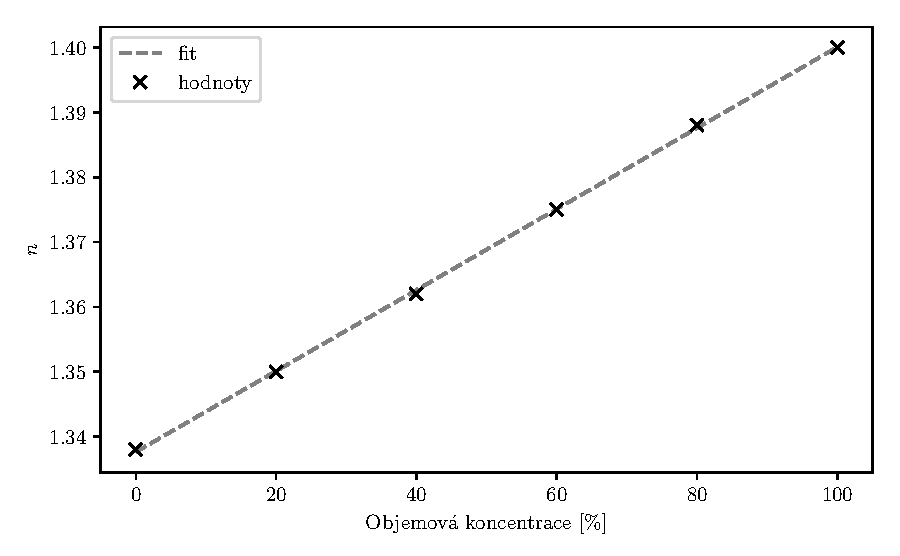
\includegraphics[]{roztok}
        \caption{Závislost indexu lomu na koncentraci roztoku}
        \label{fig:roztok}
      \end{figure}

      Byla provedena lineární regrese přímkou se směrnicí 
      $$ A = \SI{6.24 \pm 0.05 e-4}{}. $$

    \subsection*{Úkol 2}

      Nejprve byl změřen index lomu polokoule bez vzorku. Výsledky jsou shrnuty v tabulce \ref{tab:koule}.

      \begin{table}[H]
        \centering
        \setlength{\tabcolsep}{10pt}
        \begin{tabular}[t]{
  S[table-format=3.0]
  S[table-format=2.2]
  S[table-format=0.2]
} \toprule
{otočení}          & {$\theta_t$}       & {$\sigma_{\theta_t}$} \\
{$[\si{\degree}]$} & {$[\si{\degree}]$} & {$[\si{\degree}]$}    \\ \midrule
  0                & 34.62              & 0.12                  \\
 45                & 34.53              & 0.12                  \\
 90                & 34.33              & 0.12                  \\
180                & 34.37              & 0.12                  \\
225                & 34.43              & 0.12                  \\
270                & 34.63              & 0.12                  \\ \bottomrule

\end{tabular}
        \caption{Naměřené úhly průchodu polokoulí refraktometru bez vzorku}
        \label{tab:koule}
      \end{table}

      Dosazením aritmetického průměru hodnot z tabulky \ref{tab:koule} do vztahu \eqref{eq:index_lomu} získáme pro $n_i = 1$
      $$ n_{pk} = \SI{1.766 \pm 0.003}{}. $$

      Následující tabulka obsahuje hodnoty úhlů průchodu tří vzorků skel. Chyba hodnot úhlů průchodu byla určena jako $\SI{0.12}{\degree}$.

      \begin{table}[H]
        \centering
        \setlength{\tabcolsep}{10pt}
        \begin{tabular}[t]{
  S[table-format=3.0]
  S[table-format=2.2]
  S[table-format=2.2]
  S[table-format=2.2]
} \toprule
{otočení}          & {$\theta_{t,1}$}   & {$\theta_{t,2}$}   & {$\theta_{t,3}$}   \\
{$[\si{\degree}]$} & {$[\si{\degree}]$} & {$[\si{\degree}]$} & {$[\si{\degree}]$} \\ \midrule
  0                & 59.58              & 57.13              & 57.07              \\
 90                & 59.48              & 57.02              & 56.97              \\
180                & 59.55              & 57.12              & 57.00              \\
270                & 59.63              & 57.32              & 57.15              \\ \bottomrule
\end{tabular}
        \caption{Naměřené úhly průchodu polokoulí refraktometru se třemi vzorky skla}
        \label{tab:skla}
      \end{table}

      Dosazením aritmetického průměru hodnot z tabulky \ref{tab:skla} do vztahu \eqref{eq:index_lomu} získáme 
      $$ n_{i,1} = \SI{1.523 \pm 0.001}{}, $$
      $$ n_{i,2} = \SI{1.484 \pm 0.001}{}, $$
      $$ n_{i,3} = \SI{1.482 \pm 0.001}{}. $$

    \subsection*{Úkol 3}

      Polokulovým refraktometrem byly naměřeny úhly průchodu pro řádný a mimořádný směr dvojlomného vzorku při různém natočení polokoule (tedy i vzorku). Výsledky zachycuje tabulka \ref{tab:dvojlom}.

      \begin{table}[H]
        \centering
        \setlength{\tabcolsep}{10pt}
        \begin{tabular}[t]{
  S[table-format=3.0]
  S[table-format=2.2]
  S[table-format=2.2]
} \toprule
{natočení}         & {$\theta_{t, o}$}  & {$\theta_{t, e}$}  \\
{$[\si{\degree}]$} & {$[\si{\degree}]$} & {$[\si{\degree}]$} \\ \midrule
  0                & 61.77              & 62.30              \\
 20                & 61.87              & 62.10              \\
 40                & 61.87              & 61.88              \\
 60                & 61.87              & 61.87              \\
 80                & 61.70              & 61.72              \\
100                & 61.63              & 61.93              \\
120                & 61.70              & 62.08              \\
140                & 61.57              & 62.15              \\
160                & 61.63              & 62.20              \\
180                & 61.67              & 62.18              \\
200                & 61.72              & 61.93              \\
220                & 61.70              & 61.83              \\
240                & 61.72              & 61.72              \\
260                & 61.72              & 61.82              \\
280                & 61.78              & 62.05              \\
300                & 61.90              & 62.23              \\
320                & 61.85              & 62.42              \\
340                & 61.87              & 62.43              \\ \bottomrule
\end{tabular}
        \caption{Úhly průchodu pro dvojlomný vzorek}
        \label{tab:dvojlom}
      \end{table}

      Hodnoty oddělené otočením $\SI{180}{\degree}$ byly zprůměrovány a dosazeny do vztahu \eqref{eq:index_lomu}. Výsledky jsou uvedené v tabulce \ref{tab:indexy} a zobrazené v grafu \ref{fig:index_lomu}. Chyba hodnot je $\num{0.001}$.

      \begin{table}[H]
        \centering
        \setlength{\tabcolsep}{10pt}
        \begin{tabular}[t]{
  S[table-format=3.0]
  S[table-format=1.4]
  S[table-format=1.4]
} \toprule
{otočení}          & {$n_o$} & {$n_e$} \\
{$[\si{\degree}]$} & {$[]$}  & {$[]$}  \\ \midrule
  0                & 1.5553  & 1.5629  \\
 20                & 1.5564  & 1.5597  \\
 40                & 1.5563  & 1.5574  \\
 60                & 1.5564  & 1.5564  \\
 80                & 1.5552  & 1.5560  \\
100                & 1.5552  & 1.5593  \\
120                & 1.5565  & 1.5617  \\
140                & 1.5552  & 1.5635  \\
160                & 1.5558  & 1.5640  \\ \bottomrule
\end{tabular}
        \caption{Spočtené hodnoty indexů lomu pro dvojlomný vzorek}
        \label{tab:indexy}
      \end{table}

      \begin{figure}[H]
        \centering
        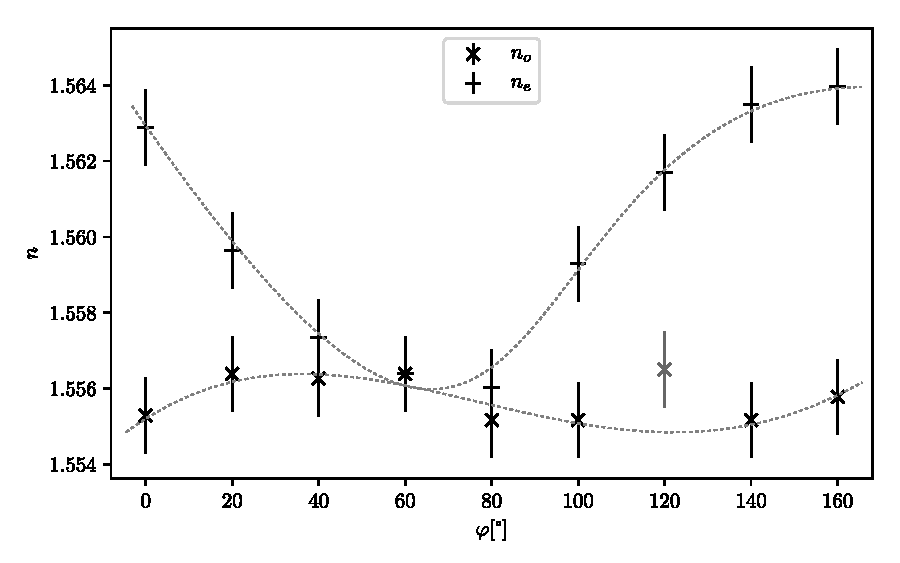
\includegraphics[]{index_lomu}
        \caption{Průběh řádného a mimořádného indexu lomu dvojlomného materiálu}
        \label{fig:index_lomu}
      \end{figure}

      Čárkované čáry v grafu slouží pouze jako vodítko pro oko, nevyjadřují analytickou závislost.

      \subsection*{Úkol 4}

        Protože mimořádný index lomu je větší než řádný, jedná se o kladný krystal.

  \section*{Diskuse}

    Z grafu \ref{fig:roztok} je vidět, že závislost indexu lomu na objemové koncentraci je s velkou přesností lineární. 

    Při měření indexu lomu skel bylo měřeno vždy několik hodnot úhlů při různém natočení vzorků. Tím se eliminoval vliv nedokonalostí tvaru skleněné polokoule refraktometru a jejího možného nedokonalého usazení. Při měření dvojlomného vzorku byly z tohoto důvodu průměrovány naměřené úhly s rozdílem otočení $\SI{180}{\degree}$.

  \section*{Závěr}

    Byl změřen index lomu kapaliny v závislosti na koncentraci.

    Byly změřeny indexy lomu skel
    $$ n_{i,1} = \SI{1.523 \pm 0.001}{}, $$
    $$ n_{i,2} = \SI{1.484 \pm 0.001}{}, $$
    $$ n_{i,3} = \SI{1.482 \pm 0.001}{}. $$

    Byly naměřeny hodnoty řádného a mimořádného indexu lomu vzorku pro různé směry šíření světla. Vzorek je kladný jednoosý krystal.

  \begin{thebibliography}{} 

    \bibitem{pokyny}
    Pokyny k měření ``Měření indexu lomu refraktometry'', dostupné z\\ \url{http://physics.mff.cuni.cz/vyuka/zfp/_media/zadani/pokyny/mereni_309.pdf}, 25.\,4.\,2018
   
  \end{thebibliography}

\end{document} 